\section{An Example Exercising P1, P2, and P3}

The labelled stochastic Petri net in Figure~\ref{fig:petri_net_log} exercises all
three problems at once: \emph{Verify Credit} (VC) and \emph{Verify Income} (VI)
are concurrent (\textbf{P2}), the \emph{Revise} (Rv) loop admits runs of unbounded
length (\textbf{P3}), and in the log the two verifications share a timestamp, so
their order is uncertain (\textbf{P1}). The net is sound, safe, and
confusion-free, as the technique requires.

\begin{figure}[h]
    \centering
    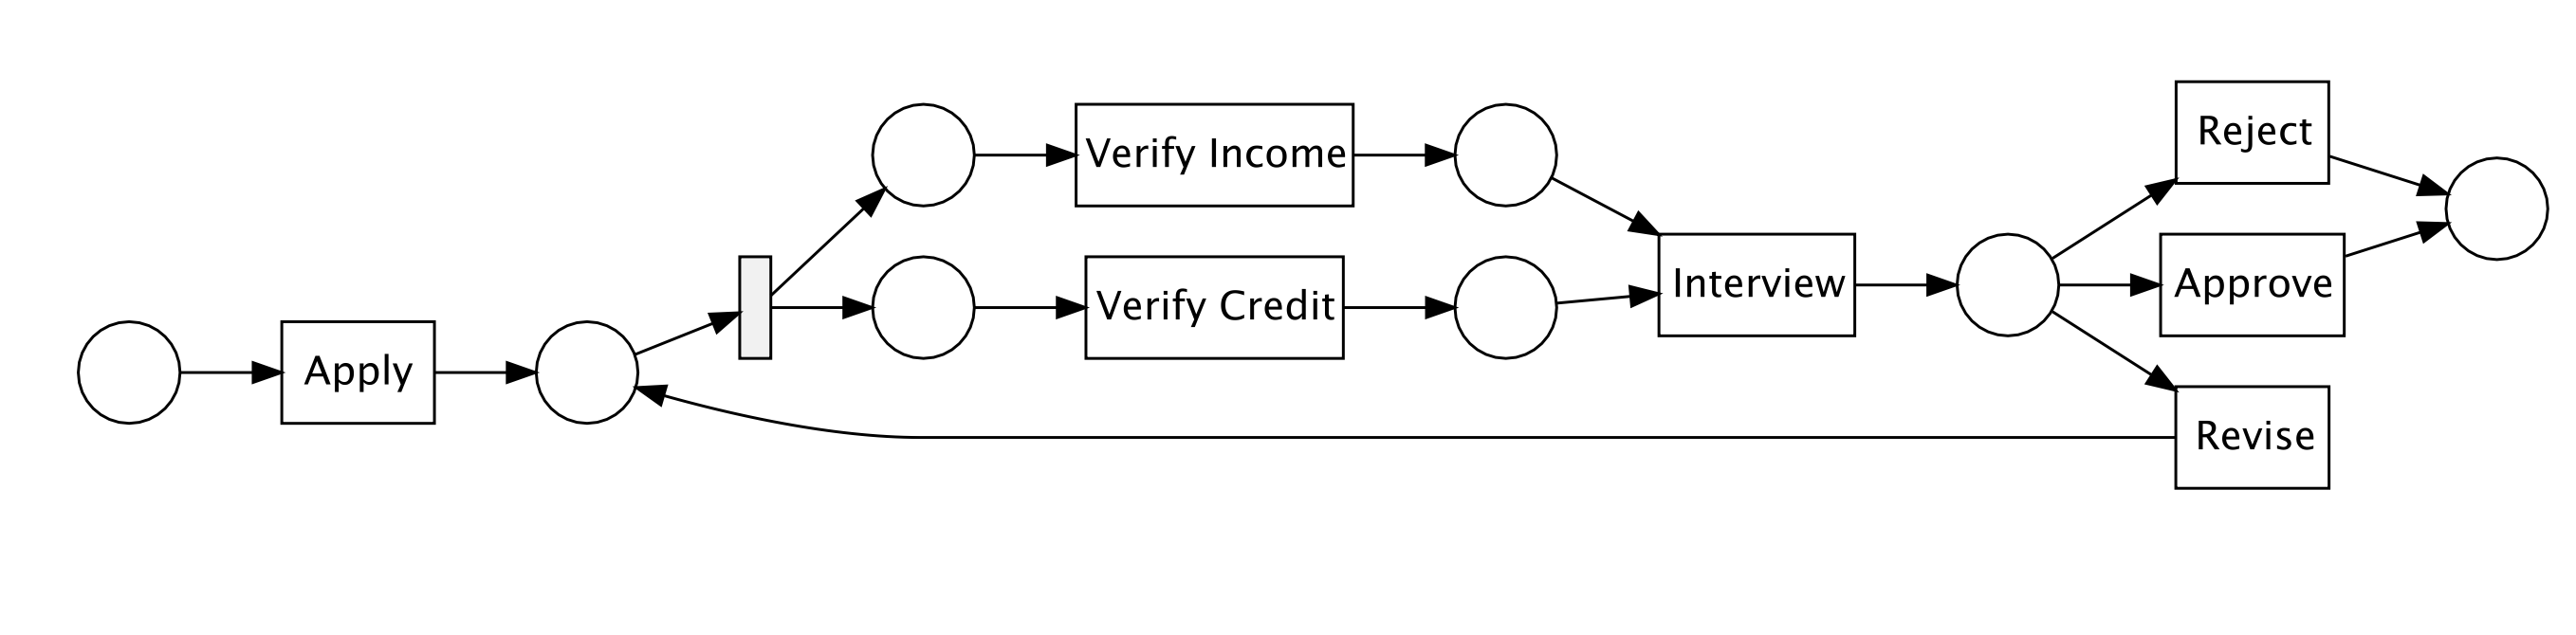
\includegraphics[width=1\textwidth]{../PMF/pics/log_petri_net.png}
    \caption{A perfectly fitting Petri net with the underlying log.}
    \label{fig:petri_net_log}
\end{figure}

The model's stochastic PO language $L_M$ is discovered from the original log
$L_1$, so it matches $L_1$ by construction. We compare it against $L_1$ and two
further logs over the \emph{same nine variants} but with different frequency
distributions: a variation log $L_2$ and a strongly loop-biased log $L_3$
(Table~\ref{tab:logs}). Under the concurrency of VC and VI the two interleavings
are linearisations of one PO trace, so the nine variants collapse into the five
PO traces $\rho_1,\dots,\rho_5$, on which $L_1$ places mass $(60,30,6,3,1)$,
$L_2$ places $(55,20,11,10,4)$, and $L_3$ places $(4,30,58,3,5)$. While $L_2$
mildly shifts mass from the short paths toward the loop, $L_3$ concentrates it
almost entirely on the looping trace $\rho_3$.

\begin{table}[h]
\centering
\footnotesize
\setlength{\tabcolsep}{4pt}
\renewcommand{\arraystretch}{1.15}
\begin{tabular}{l c r r r}
\hline
\textbf{Trace variant} & \textbf{PO trace} & $\mathbf{L_1}$ & $\mathbf{L_2}$ & $\mathbf{L_3}$ \\
\hline
$\langle \text{A}, \text{VC}, \text{VI}, \text{I}, \text{Ap}\rangle$ & $\rho_1$ & 30 & 15 & 1 \\
$\langle \text{A}, \text{VI}, \text{VC}, \text{I}, \text{Ap}\rangle$ & $\rho_1$ & 30 & 40 & 3 \\
$\langle \text{A}, \text{VC}, \text{VI}, \text{I}, \text{R}\rangle$ & $\rho_2$ & 16 & 10 & 1 \\
$\langle \text{A}, \text{VI}, \text{VC}, \text{I}, \text{R}\rangle$ & $\rho_2$ & 14 & 10 & 29 \\
$\langle \text{A}, \text{VC}, \text{VI}, \text{I}, \text{Rv}, \text{VC}, \text{VI}, \text{I}, \text{Ap}\rangle$ & $\rho_3$ & 3 & 6 & 1 \\
$\langle \text{A}, \text{VI}, \text{VC}, \text{I}, \text{Rv}, \text{VI}, \text{VC}, \text{I}, \text{Ap}\rangle$ & $\rho_3$ & 3 & 5 & 57 \\
$\langle \text{A}, \text{VC}, \text{VI}, \text{I}, \text{Rv}, \text{VC}, \text{VI}, \text{I}, \text{R}\rangle$ & $\rho_4$ & 2 & 5 & 2 \\
$\langle \text{A}, \text{VI}, \text{VC}, \text{I}, \text{Rv}, \text{VI}, \text{VC}, \text{I}, \text{R}\rangle$ & $\rho_4$ & 1 & 5 & 1 \\
$\langle \text{A}, \text{VI}, \text{VC}, \text{I}, \text{Rv}, \text{VI}, \text{VC}, \text{I}, \text{Rv}, \text{VI}, \text{VC}, \text{I}, \text{Ap}\rangle$ & $\rho_5$ & 1 & 4 & 5 \\
\hline
\textbf{Total} & & \textbf{100} & \textbf{100} & \textbf{100} \\
\hline
\end{tabular}
\caption{Variant frequencies of the original log $L_1$, the variation log $L_2$,
and the loop-biased log $L_3$ (each $100$ traces). A = Apply, VC = Verify Credit,
VI = Verify Income, I = Interview, Rv = Revise, Ap = Approve, R = Reject.}
\label{tab:logs}
\end{table}

Using the \href{https://leemans.ch/ebi/index.php}{Ebi} CLI, I sampled the model's
partially ordered traces (\texttt{ebi sample partially-ordered-traces}, $1000$
runs) and computed EMSC against each log. $L_1$ scored $0.996$; the missing
$0.004$ is the residual mass $L_M(\bot)$ left by truncating the loop
(\textbf{P3}). $L_2$ scored $0.926$ and $L_3$ only $0.744$, since the transport
must move their loop-heavy mass onto the short traces $L_M$ favours: the more a
log departs from $L_M$, the more mass travels at a positive PO-trace distance.
The ordering $\mathrm{emsc}(L_M, L_3) = 0.744 < 0.926 = \mathrm{emsc}(L_M, L_2) <
0.996 = \mathrm{emsc}(L_M, L_1)$ confirms that $L_3$ is stochastically furthest
from the model.
